\documentclass[ngerman,compress,hyperref={bookmarks}]{beamer}
%\usetheme{Frankfurt}
%\usetheme{boxes}
%\usetheme{Malmoe}
\usetheme{Antibes}
%\useoutertheme{infolines}
%\useoutertheme{split}
\usepackage[utf8x]{inputenc}
%\usepackage[nolist]{acronym}

\usepackage{colortbl}
\definecolor{dunkelgrau}{rgb}{0.8, 0.8, 0.8}

\usepackage{wasysym}

%\logo{
\includegraphics[height=1cm]{logoHAW}}
\usepackage{graphicx}
%\usepackage[%
%	bibstyle=authoryear,%
%	citestyle=authoryear,%
%	bibencoding=utf8,%
%	bibtex8=true,%
%	sorting=nyt,%
%	sortcites=true,%
%	maxnames=2,%
%	babel=other,%
%	block=space,%
%	backref=false,%
%	natbib=true,%
%	hyperref=true,%
%]{biblatex}
%\bibhang1em
%\usepackage[style=authortitle-icomp]{biblatex}
%\bibliography{routing_atlas}

\setbeamertemplate{bibliography entry title}{}
\setbeamertemplate{bibliography entry location}{}
\setbeamertemplate{navigation symbols}{} 
\setbeamertemplate{footline}[page number]

\title{Lernen und Wissen in Unternehmen}
\subtitle{Vortrag: Unternehmensorientierung}
\subject{}
\author{Benjamin Vetter \and Andreas Krohn}
\institute[HAW]{Hochschule für Angewandte Wissenschaften Hamburg}
\date[WS 2011/12]{11. Januar 2012}

\begin{document}

\section{Lernen im Unternehmen}

\frame{\titlepage}

\frame{
  \frametitle{Agenda}

  \tableofcontents
}

\frame{
  \frametitle{Lernen: Eine Definition}

  Was ist ,,lernen''?

  \begin{itemize}
    \item
  \end{itemize}
}

\subsection{Motivation und Problematik}

\frame{
  \frametitle{Motivation}

  \begin{block}{Lernen im Unternehmen - Warum?}
    Das Unternehmen als Individuum, sich selbst organisierende und gestaltende
    soziale Handlungseinheit
  \end{block}

  \vspace{0.5cm}

  \begin{columns}
    \column{0.68\textwidth}
      Worum geht es dabei?

      \begin{itemize}
        \item Lernprozesse der Mitarbeiter initiieren und steuern
        \item Individuelles und Gruppenlernen
      \end{itemize}

      \vspace{0.5cm}

      $\rightarrow$ Individuelles Lernen \\
      \hspace{0.1cm} $\rightarrow$ Austausch, Interaktion, Harmonisierung \\
      \hspace{0.2cm} $\rightarrow$ Gruppenlernen

    \column{0.35\textwidth}
      
\includegraphics[width=1\textwidth]{images/learning-company.png}
  \end{columns}
}

\frame{
  \frametitle{Herausforderungen 1}

  \begin{columns}
    \column{0.55\textwidth}
      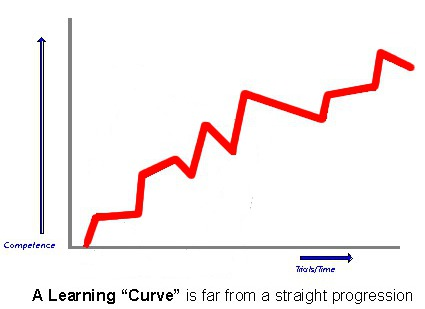
\includegraphics[width=1\textwidth]{images/learning-curve.jpg}

    \column{0.55\textwidth}
      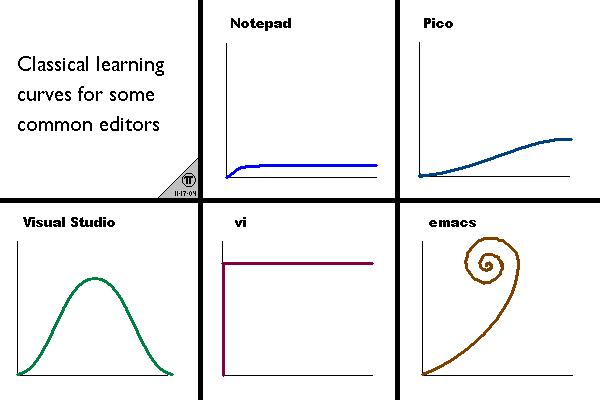
\includegraphics[width=1\textwidth]{images/curves.jpg}
  \end{columns}

  \footnotetext[1]{\tiny \url{http://www.learningandteaching.info/learning/learning_curve.htm} \cite{curve1}}
  \footnotetext[2]{\tiny \url{http://www.terminally-incoherent.com/blog/2006/08/01/text-editor-learning-curves/} \cite{curve2}}
}

\frame{
  \frametitle{Herausforderungen 2}

  ,,We might already be beyond the age of speed, by moving into the age of real-time.''
  - Ivan Illich, Austrian philosopher (1926-2002)

  Weitere Herausforderungen:

  \begin{itemize}
    \item Gruppenverhalten und -Rollen \cite{Huebner:2011}
      % Verschiedene Erwartungen, potentielle Konflikte, unterschiedliche Wahrnehmung (Konstruktivismus)
    \item Konstruktivismus \cite{Watzlawick:1992}
  \end{itemize}
}

\frame{
  \frametitle{Das Unternehmen als Individuum}

  \begin{itemize}
    % \item Möglich, aufgrund langfristiger Erreichung gemeinsamer Ziele
    \item Analogie um Lernprozesse im Unternehmen besser nachvollziehen zu können
    \item Unternehmskultur entspricht der Persönlichkeit
    \item Das unternehmerische Handeln ist das bewusste Tun, wodurch es sich selbst oder seine Umwelt verändert
    \item Die Wissensbasis bestimmt das Handeln
    \item Dessen Konsequenzen initiieren den Lernprozess
    \item Der Lernprozess verändert die Wissensbasis
  \end{itemize}

  \begin{block}{Resultat}
    Bessere Systemanpassung und Problemlösungsfähigkeit
  \end{block}

  % Beispiel
}

\frame{
  \frametitle{Das lernende Unternehmen: in der Vergangenheit}

  \begin{columns}
    \column{0.65\textwidth}
      Beginn der Disziplin:

      \begin{itemize}
        \item 1950-60er Jahre
        \item Passive Rolle des Unternehmens
        \item Ausschließlich ,,Reagieren''
      \end{itemize}

    \column{0.35\textwidth}
      
\includegraphics[width=1\textwidth]{images/buecher.jpg}
  \end{columns}

  ... Abstecher in die Theorien
}

\subsection{Organisationale Lerntheorien}

\frame{
  \frametitle{Cyert und March}

  Cyert und March:

  \begin{itemize}
    \item Vorher: Unternehmen als rationales, über alle notwendigen Informationen verfügendes System
    \item Cyert und March: Unternehmen als adaptives, sich anpassendes rationales System
          % potentiell verschiedene Systemzustände
          % effektiv realisierter Zustand durch Umwelteinflüsse und eigene Ziele gesteuertes Verhalten bestimmt
  \end{itemize}

  Grundlegene Prinzipien:

  \begin{itemize}
    \item Vermeide Unsicherheit
    \item Halte an bewährten Regelsystemen fest
    \item Benutze einfache Regeln
  \end{itemize}
}

\frame{
  \frametitle{Argyris und Schön}

  Argyris und Schön:

  \begin{itemize}
    \item Unternehmerisches Handeln als individuelles durch Rollen geleitetes Handeln
    \item Geäußerte Handlungstheorien VS reale Gebrauchstheorien
    \item Diskrepanzen initiieren Lernprozesse
    \item Drei Lerntypen
      \begin{itemize}
        \item Single-Loop
          % Zielabweichungen werden erkannt und korrigiert
          % Nur Anpassung der Parameter in vorgegebenem Schemata
          % Beispiel: Sinkender Absatz erfordert mehr Werbung und Verkaufsaktivitäten
        \item Double-Loop
          % Lernen durch Bewertung und Entwicklung von Schemata
          % Modifikation und Verbesserung der allgemeinen Regeln, Normen und Ziele
          % Quasi: Ursachenanalyse
          % Beispiel: sinkender Absatz führt zur Überprüfung, ob dies an zu wenig Werbung oder mangelnder Produktqualität liegt
        \item Deutero
          % Lernendes Lernen, höchstes Lernniveau
          % Selbstreflexion der Lernprozesse, mit Wissen aus vergangenen Lernprozessen
      \end{itemize}

      % Wenn Double-Loop oder Deutero Lernen nicht erreicht wird können die Ursachen bspw. in defensivem Verhalten der Miterbeiter liegen
      % und dem Wunsch negative Gefühle zu vermeiden. Probleme werden dann vertuscht und unterdrückt um vor negativen Gefühlen zu schützen.
  \end{itemize}

  Erfordert offene und konstruktive Lern- und Diskussionskultur
}

\frame{
  \frametitle{P. Senge}

  \begin{block}{Unternehmen sind}
    ,,ein Ort, an dem Menschen kontinuierlich entdecken, dass sie ihre Realität
    selbst erschaffen. Und dass sie sie verändern können.''
  \end{block}

  \vspace{0.3cm}

  Sieben Hindernisse:

  \vspace{0.3cm}

  \begin{columns}
    \column{0.6\textwidth}
      \begin{itemize}
        \item Ich bin meine Position
        \item Der Feind da draußen
        \item Angriff ist die beste Verteidigung
        \item Fixierung auf Ereignisse
      \end{itemize}

    \column{0.6\textwidth}
      \begin{itemize}
        \item Gleichnis vom gekochten Fisch
        \item Illusion aus Erfahrung zu lernen
        \item Mythos vom Managementteam
      \end{itemize}
  \end{columns}
}

\frame{
  \frametitle{,,Fünf Disziplinen'' als Lösung}

  \begin{center}
    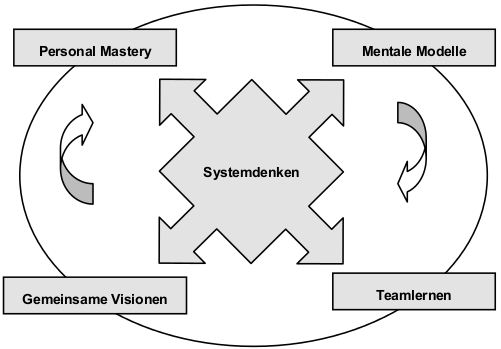
\includegraphics[width=0.8\textwidth]{images/senge.png}
  \end{center}
}

\frame{
  \frametitle{Das lernende Unternehmen: im Jetzt}

  Nur ein lernfähiges Unternehmen kann in einer Wissensgesellschaft erfolgreich
  sein. \cite{Franken:2007}

  \vspace{0.3cm}

  Nonaka und Takeuchi:

  \begin{itemize}
    \item Schaffung neuen Wissens steht über Wissensverarbeitung
    \item Ständige Erneuerung der Denk- und Handlungsmodelle
    \item Lerndimensionen im Unternehmen:
    \begin{itemize}
      \item Epistemologische Dimension: explizites und implizites Wissen
      \item Ontologische Dimension: Individuum und Kollektiv
    \end{itemize}
  \end{itemize}

  Nur Einzelpersonen erzeugen Wissen. Das Unternehmen muss deren Kreativität
  unterstützen, und im Wissensnetz verankern.
}

\frame{
  \frametitle{Nonaka und Takeuchi: die vier Dimensionen}

  \begin{center}
    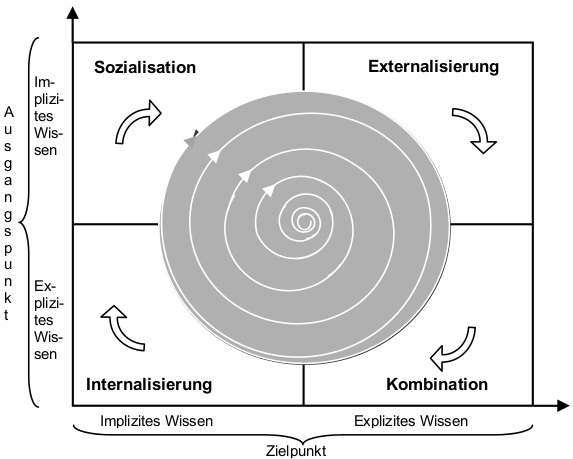
\includegraphics[width=0.8\textwidth]{images/nonaka.png}
  \end{center}

  % Verschiedene Phasen der Wissensgewinnung:
  % - Wissen austauschen
  % - Konzepte schaffen
  % - Konzepte erklären
  % - Einen Archetyp bilden
  % - Wissen übertragen

  % Verschiedene Vorraussetzungen:
  % - Intention
  % - Autonomie
  % - Redundanz
  % - Fluktuation und kreatives Chaos
  % - Notwendige Vielfalt
}

\subsection{Kritik}

\frame{
  \frametitle{Das lernende Unternehmen: in der Zukunft}

  Meine Bewertung: die Theorien gehen nicht weit genug

  \begin{itemize}
    \item Welche Arbeitsbedingungen sind förderlich fürs Lernen
    \item Konstruktivismus \cite{Watzlawick:1992}
    \item Auswirkungen der Lernkultur
    \item Umgang mit Fehlern, Fehlerkultur
    \item Digitales Zeitalter
  \end{itemize}
}

\frame{
  \frametitle{Konnektivismus}

  Konnektivismus:

  \begin{itemize}
    \item Der Mench wird nicht länger als ,,isoliertes'' Wesen betrachtet
    \item Zugriff auf verschiedene Netzwerke möglich
  \end{itemize}
}

\frame{
  \frametitle{Lernkultur}

  \begin{center}
    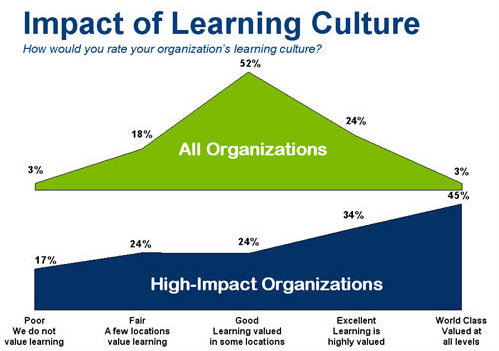
\includegraphics[width=0.8\textwidth]{images/culture.jpg}
  \end{center}

  \footnotetext[1]{\tiny \url{http://joshbersin.com/2008/08/13/the-hilo-80-leaders-in-corporate-learning/} \cite{culture}}
}

\subsection{Zusammenfassung}

\frame{
  \frametitle{Zusammenfassung}
}




%\frame{\titlepage}

\section{Wissen im Unternehmen}

\frame{
  \frametitle{Agenda}

  \tableofcontents
}

% Bedingt durch Globalisierung, Wettbewerb und Informationstechnik streben Unternehmen danach hochwertige Produkte und Dienstleistungen anzubieten
% Verschiebung d. Wirtschaft hin zum tertiären Sektor (Dienstleistungen) ~ 1950 32,5% \ldots 1975 51,0% \ldots 2011 73,8% (lt. Statistischem Bundesamt)
% Dafür sind die Mitarbeiter und deren Fähigkeiten die wichtigste Resource - Sie verfügen über ``Wissen''

\subsection{Einführung}
\frame{
  \frametitle{Einführung}
      Was ist Wissen?\\
      \vspace{0.2cm}
      Nur näherungsweise und im Kontext zu definieren\\
      \vspace{0.2cm}
      Ansätze:
      \begin{itemize}
         \item Nach Zugänglichkeit: Implizites und explizites Wissen
         \item Nach Personeller Bindung: Individuelles und kollektives Wissen
         \item Wissen vs. Information vs. Daten\\
           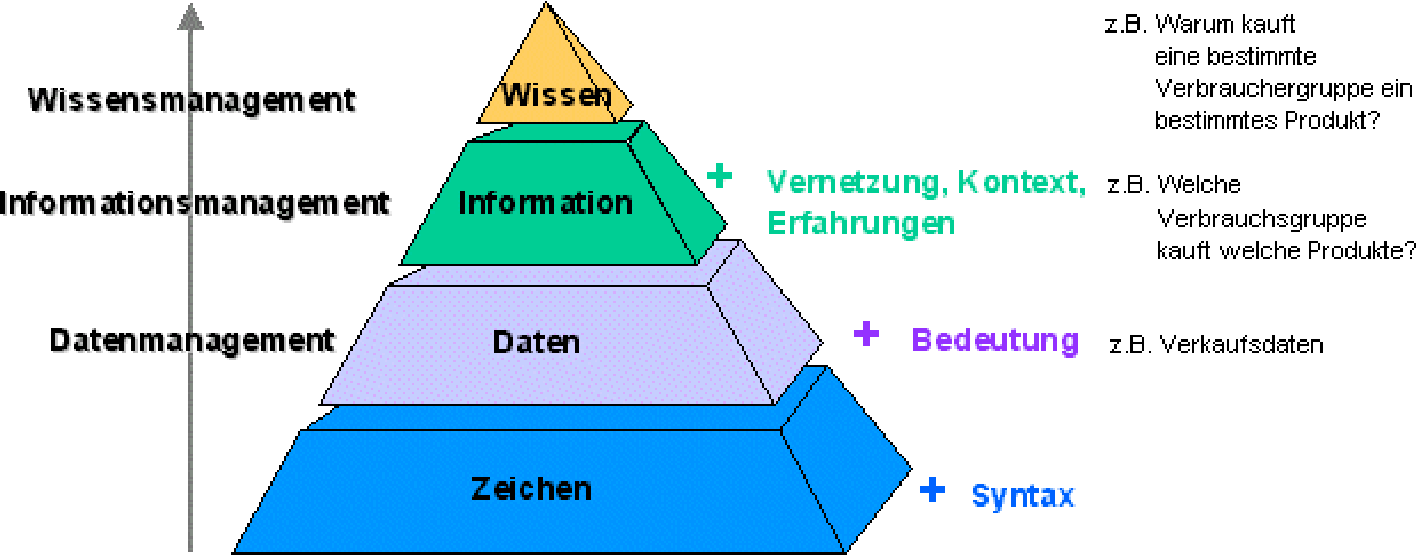
\includegraphics[width=0.5\textwidth]{images/wissenspyramide.png}
         \item ``Wissen ist in einen Kontext eingebettet und von ihm abhängig und kann daher nicht zeitlos objektiv sein.'' \cite{Schilcher:2006}
      \end{itemize}
  \vspace{0.1cm}  
  \begin{center}\small``Ich weiß, dass ich nichts weiß'' - Sokrates\end{center}
}
% ``Ich weiß, dass ich nicht[s] weiß'' ~ Sokrates
% Eine Definition des Begriffs ``Wissen'' ist kaum zu finden bzw. je nach Kontext und Autor verschieden
% Ansätze: 
% - Zugänglichkeit: Implizites und Explizites Wissen
% - Personelle Bindung: Individuelles und Kollektives Wissen
% - Wissen vs. Information (Sachverhalt unter best., def. Randbed. [Schmiede 1996a]) vs. Daten [vs. Zeichen]
%	Beispiel: Hilferuf am Badesee, Wechselkurs und Leitzinsänderungen
% - Wissen ist nicht ahistorisch, von sozialen & kulturellen Umständen abhängig (z.B. Maßeinheiten) ~ ``Wissen ist in einen Kontext eingebettet und von ihm abhängig und kann daher nicht zeitlos objektiv sein.'' [S. 18, Schilcher, C. - Implizite Dimensionen des Wissens und ihre Bedeutung für betriebliches Wissensmanagement, 2006]

\frame{
  \frametitle{Hauptformen des Wissens im Unternehmen}
  Hauptformen des Wissens im Unternehmen nach Franken \cite{Franken:2002}
  \begin{itemize}
    \item \textbf{Strukturiertes, formalisiertes Wissen} explizit und strukturiert, z.B. Datenbanken, ausgefüllte Formulare
    \item \textbf{Unstrukturiertes, formalisiertes Wissen} explizit und unstrukturiert, z.B. Bilder, Baupläne
    \item \textbf{Personelles Wissen} implizit, an Personen gebunden und durch Kommunikation vermittelbar
    \item \textbf{Kollektives Wissen} implizites, kulturelles Wissen
  \end{itemize}
  $\rightarrow$ Probleme im Umgang mit impliziten Wissensformen
}
% Franken: Hauptformen des Wissens in Unternehmen [Franken, Integriertes Knowledge Management]
% (S. 303)
% 1- Strukturiertes Wissen
% 2- Unstrukturiertes, formalisiertes Wissen
% 3- Personelles, individuelles Wissen
% 4- Kollektives Wissen
% Umgang mit 3 & 4 im Unternehmen nicht einfach -> Wissensmanagement erforderlich (wieder..)

\subsection{Motivation: Wissensmanagement}
\frame{
  \frametitle{Motivation: Wissensmanagement}
  Wozu Wissensmanagement?\\ \vspace{0.3cm}
  \begin{itemize}
    \item Kosten für externe Dienstleistungen verringern
    \item Verhindern doppelter Arbeit in verschiedenen Abteilungen
    \item Wissen im Unternehmen halten (auch bei Kündigung, Pensionierung, \ldots)
    \item Problemen des impliziten Wissens begegnen
  \end{itemize}
  
}
% Wozu Wissensmanagement? (S. 304)
% - Kompetenzen der Mitarbeiter kennen, nutzen (und ausbauen)..
%	.. da sonst:
%		- externe Dienstleistungen bezahlt werden, die In-House erledigt werden können
% - Austausch von Wissen innerhalb des Unternehmens..
%	.. da sonst:
%		- eine Abteilung etwas entwickelt, das eine andere Abteilung bereits fertiggestellt hat
% - IMHO Wichtigster Punkt:
% 	Sicherstellen, dass bei Kündigung, Pension etc. das Wissen im Unternehmen bleibt.
% -> Problemfall implizites Wissen
% 	Wie motiviere ich meine Mitarbeiter, Wissen weiterzugeben und von anderen anzunehmen?
% 		- Ideen sammeln? (Fragerunde?, Erfahrungen?, ..)
%		- Beispiel: Stellenabbau, Wissen über Verfahren weitergeben, aber an wen? und wie?
%		- ``Wissen ist Macht'' <-> Klima ausreichender Sicherheit und Offenheit schaffen, damit 'Hoheitswissen' geteilt wird

\frame{
  \frametitle{Kulturelle Unterschiede und der Wert des Impliziten}
  Nonaka und Takeuchi \cite{Nonaka:1997}
  \begin{itemize}
    \item In westlichen Unternehmen ist ``Wissen'' vor allem explizit.
    \item Japanische Unternehmen legen mehr Wert auf Implizites,\\
          z.B. Erfahrung, Intuition
  \end{itemize}
  \begin{center}
    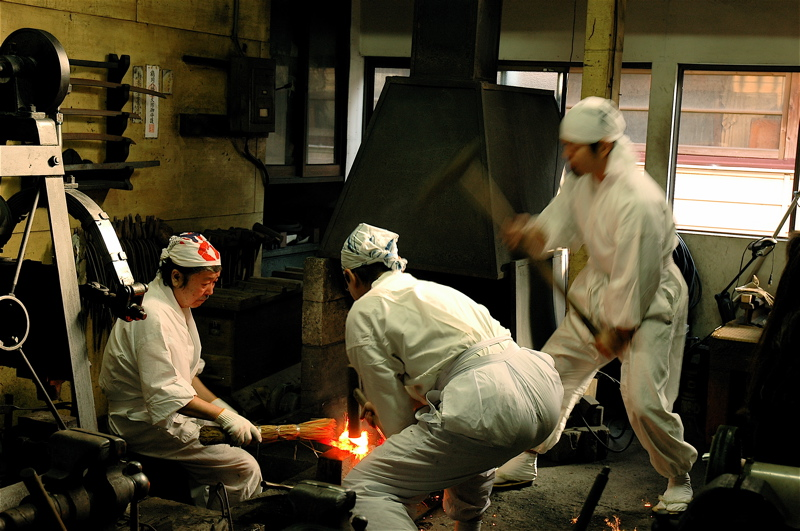
\includegraphics[width=0.6\textwidth]{images/kamakura-masamune-swordsmith-1.jpg} \cite{samurai}
  \end{center}
}
% Nonaka und Takeuchi: Kulturelle Unterschiede
% - Für westl. Unternehmen ist Wissen explizit. ``Explizites Wissen lässt isch in Worten und Zahlen ausdrücken und problemlos mit Hilfe von Daten, wissenschaflichen Formeln, festgelegten Verfahren oder universellen Prinzipien mitteilen'' [Nonake, Takeuchi, Die Organisation des Wissens]
% - Japan. Unternehmen ist der Stellenwert impliziten Wisses deutlich höher. ``Subjektive Einsichten, Ahnungen und Intuition fallen in diese Wissenskategorie. Darüber hinaus ist das implizite Wissen tief verankert in der Tätigkeit und deer Erfahrung des einzelnen sowie in seinen Idealen, Werten und Gefühlen'' [s.o.]

\subsection{Wissensmanagement}
\frame{
  \frametitle{Probst, Raub, Romhardt - Bausteine des Wissensmanagements \cite{Probst:2006}}
  \begin{columns}
    \column{0.5\textwidth}
      Gliederung in die Kernelemente
      \begin{itemize}
        \item Wissensidentifikation
        \item Wissenserwerb
        \item Wissensentwicklung
        \item Wissens(ver)teilung
        \item Wissensnutzung
        \item Wissensbewahrung
      \end{itemize}

    \column{0.5\textwidth}
      Ergänzt durch
      \begin{itemize}
        \item Wissensziele
        \item Wissensbewertung
      \end{itemize}

      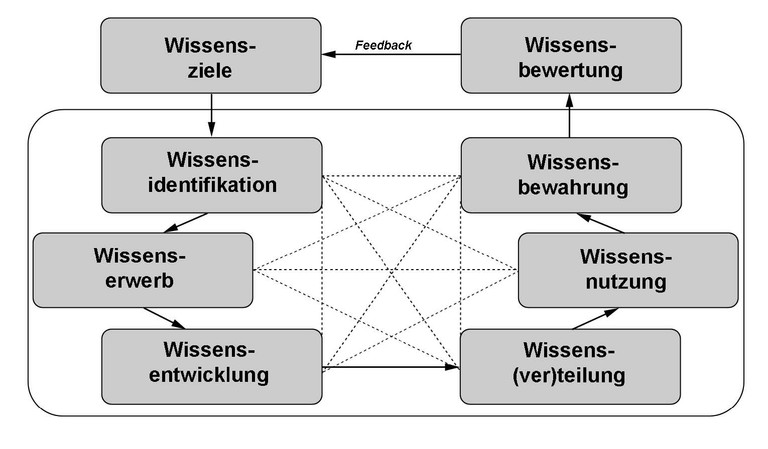
\includegraphics[width=0.8\textwidth]{images/probst.jpg}
  \end{columns}

  \begin{alertblock}{Kritik: Praxistauglichkeit}
    Hinweise zur Umsetzung fehlen. Wissensbewertung?
  \end{alertblock}
}
% G. Probst, S. Raub, K. Romhardt: ``Bausteine des Wissensmanagements'' [ebd. Wissen managen]
% Kernelemente: (S. 304)
% - Wissensidentifikation
% - Wissenserwerb
% - Wissensentwicklung
% - Wissens(ver)teilung
% - Wissensnutzung
% - Wissensbewahrung
% beschreiben die operativen Probleme des Umgangs mit Wissen im Unternehmen
% weiterhin
% - Wissensziele: Normativ (wissensbewusste Unternehmenskultur), Strategisch (zukünftigen Wissensbedarf definieren), Operativ (Umsetzung d. Wissensmanagement)
% - Wissensbewertung: Metriken, Bewertungskriterien finden, um Grad der Erfüllung o.g. Ziele zu messen \ldots nur wie?
% Kritik: Keine Hinweise auf praktische Umsetzung; Wissensbewertung (nahezu) unmöglich

\frame[allowframebreaks]{
  \frametitle{Wissensmanagement in der Praxis}
  Franken \cite{Franken:2007}
  \begin{itemize}
    \item Mitarbeiter steht im Mittelpunkt
    \item Voraussetzungen für freiwilliges Engagement schaffen
    \item Verhaltenskomponenten
      \begin{itemize}
        \item sollen
        \item dürfen
        \item können
        \item wollen
      \end{itemize}
  \end{itemize}
  Es bedarf der ``Befähigung, Fähigkeit und Bereitschaft zu lernen, Wissen anzunehmen sowie eigenes Wissen zu teilen'' \cite{Franken:2007}
  \framebreak

  Arbeitsbereiche des praktischen Wissensmanagements
  \begin{enumerate}
    \item \textbf{Wissensvision schaffen}
    \begin{itemize}
      \item Bild der Zukunft des Unternehmens vermitteln $\rightarrow$ ``sollen''
      \item Identifikation mit dieser Zukunft soll zu Engagement motivieren $\rightarrow$ ``wollen''
    \end{itemize}
    \item \textbf{Wissensgemeinschaft bilden}
    \begin{itemize}
      \item Förderung des individuellen Lernens z.B. in Workshops $\rightarrow$ ``können''
      \item Positive Einstellung gegenüber Neuerungen, Angstfreiheit, ``sinnvolle Fehlschläge'' tolerieren $\rightarrow$ ``dürfen''
    \end{itemize}
\framebreak
    \item \textbf{Interaktion unterstützen}
    \begin{itemize}
      \item Wissensaustausch fördern
      \item Offene Kommunikation und Vertrauen schaffen
    \end{itemize}
    \item \textbf{Erneuerungen fördern}
    \begin{itemize}
      \item Neue Teams zusammenstellen
      \item Nichtexperten einsetzen
      \item Ziel: Betrachtungsweisen in Frage stellen und neue gewinnen
    \end{itemize}
    \item \textbf{Middle-up-down-Management}
    \begin{itemize}
      \item Mittelweg zwischen hierarchischem und partizipativem Führungsstil
      \item ``Das implizite Wissen von oben (Visionen) und unten (Erfahrungen, Fertigkeiten und Intuition) verschmilzt und wird zum expliziten Wissen in Form von neuen Technologien, Produkten oder Programmen.'' \cite{Franken:2007}
    \end{itemize}
    \item \textbf{Hypertextorganisation}
    \begin{itemize}
      \item Vorteile von Bürokratie (Sammeln, Formalisieren von Wissen) und Arbeitsgruppe (Flexibilität, Generieren von Wissen) nutzen
      \item Zusammenfassung des Wissens in Wissensbasis
    \end{itemize}
    \item \textbf{Wissensnetz mit der Außenwelt}
    \begin{itemize}
      \item Wissen externer Interessengruppen erschließen und benutzen
      \item Keyuser in Produktentwicklung einbinden
      \item Forschungskooperationen
    \end{itemize}
  \end{enumerate}
}
% Franken (in Anlehnung an Nonaka und Takeuchi) - Wissensmanagement in der Praxis
% Voraussetzungen für das Verhalten der Mitarbeiter schaffen 
% ~ Verhaltenskomponenten:
%	``sollen'', ``dürfen'', ``können'' und ``wollen''
% - Mitarbeiter stehen im Mittelpunkt d. Wissensmanagements
% - Bedarf d. ``Befähigung, Fähigkeit und Bereitschaft zu lernen, Wissen anzunehmen sowie eigenes Wissen zu teilen'' [Franken, S. 307]
% - 

\subsection{Das intelligente Unternehmen}
\frame{
  \frametitle{Das intelligente Unternehmen}

  Anwendung des klassischen, individuellen Intelligenzbegriffs auf Unternehmen

  \begin{itemize}
    \item \emph{Kognitive Intelligenz}: Informationsaufnahme, Bewertung, schlussfolgerndes Denken, Lernen aus Erfahrung, Bewältigung neuer Situationen und optimale Gestaltung der Umwelt
    \item \emph{Soziale Intelligenz}: Intern, im Bezug auf Mitarbeiter und extern, im Bezug auf Kunden, Lieferanten und Umwelt
    \item \emph{Technische Intelligenz}: Materielle, räumliche und technologische Beschaffenheit des Unternehmens
  \end{itemize}

  Wissenslogistik befähigt ein Unternehmen vorhandenes Wissen zu nutzen

  Harmonisierung widersprüchlichen Wissens führt zur Bildung einer Unternehmensidentität
}

\subsection{Fazit \& Praxistipps}
\frame{
  \frametitle{Tools, Maßnahmen}

  \begin{columns}
    \column{0.6\textwidth}
      \begin{itemize}
        \item Bewusstsein für vorhandenes Wissen schaffen
%        \item Dokumentation
        \item Wikis, Stackoverflow, Blogs, \ldots
%        \item Kommunikation
        \item Vorträge von internen und externen Experten
        \item Einbeziehung fachfremder Personen
        \item Aufgeschlossenheit gegenüber Kreativität und Neuerungen
%        \item ``Wissen ist Macht'' überwinden
      \end{itemize}

    \column{0.4\textwidth}
      
\includegraphics[width=0.5\textwidth]{images/wordpress.pdf} \\
      \vspace{0.5cm}
      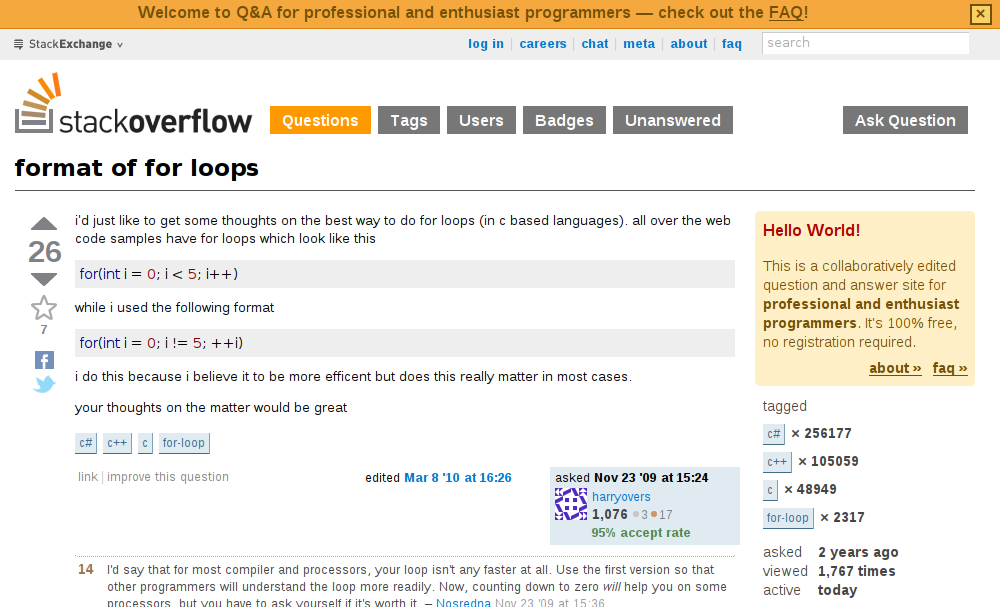
\includegraphics[width=0.8\textwidth]{images/stackoverflow.png}\\
      \vspace{-0.5cm}
      \hspace{0.5cm}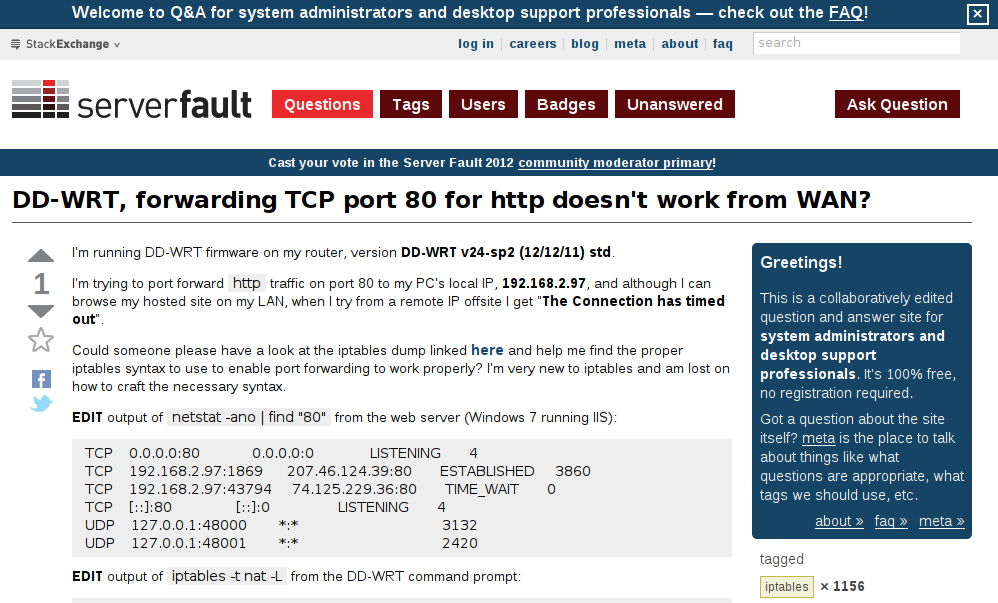
\includegraphics[width=0.8\textwidth]{images/serverfault.png}\\
  \end{columns}
}

\frame{
  \frametitle{Fazit}
%    \begin{itemize}
%      \item Implizite Wissen verteilen und (wenn möglich) formalisieren
%      \item Aufgeschlossenheit gegenüber Kreativität und Neuerungen 
%      \item ``Tools'' z.B. Wikis, Blogs, stackoverflow, \ldots
%      \item Events als Kommunikationsgelegenheit
%      \item Vorträge von Mitarbeitern für Mitarbeiter
%      \item \ldots
%    \end{itemize}
}
%\subsection{Einführung}
%\frame{
%  \frametitle{Einführung}
%  \begin{itemize}
%    \item Trend zur Wissensarbeit
%    \item ``Immaterielle'' Wertschöpfung
%    \item Metapher: Fabrik $\rightarrow$ Küche
%  \end{itemize}
%}

%\subsection{Definition: Wissen}
%\begin{frame}[allowframebreaks]
%\frametitle{Definition: Wissen}
%\begin{description}
% \item[Zeichen] Symbole, kontextfrei
% \item[Daten] Verkettung von Zeichen, frei von einem Verwendungszweck
% \item[Informationen] Daten im Kontext eines Problemzusammenhangs
% \item[Wissen] Eine Menge von Informationen, Modellierte Wirklichkeit
%\end{description}
%\textbf{Beispiel}: Wechselkurse %``1'' ``,'' ``4'' ``9'' $\rightarrow$ ``1,49'' $\rightarrow$ ``1,49 EUR/USD'' $\rightarrow$ Verhalten von Kursen angesichts von Leitzins, Markt, \ldots
%\framebreak
%\begin{description}
% \item[Explizit] Regeln, Texte
% \item[Implizit] Intuitives Handeln, Wiedererkennen bekannter Situationen
%\end{description}
%\end{frame}

%\subsection{Wissensgenerierung}
%\begin{frame}{Wissensgenerierung}
%Intern
%\begin{itemize}
% \item Forschung und Entwicklung
% \item Anreize zum Wissenstransfer
% \item Technische Infrastruktur
%\end{itemize}
%Extern
%\begin{itemize}
% \item Forschungskooperationen
% \item Lead-User
% \item Lieferanten-Kunden-Netzwerk
%\end{itemize}
%\end{frame}





\section{Referenzen}

\begin{frame}[allowframebreaks]{Referenzen}
\bibliographystyle{plain}
\bibliography{folien.bib}
\end{frame}

\end{document}


